\documentclass[11pt,letter]{article}
\usepackage{amsmath}
\usepackage{amssymb}	% packages that allow mathematical formatting
\usepackage{graphicx}	% package that allows you to include graphics
\usepackage{setspace}	% package that allows you to change spacing
\usepackage{fullpage}	% package that specifies normal margins
\usepackage{microtype}
\usepackage{amsthm}
\newcommand{\argmin}{\operatornamewithlimits{argmin}}
\renewcommand\qedsymbol{$\blacksquare$}
\usepackage{listings}
\usepackage{color}
\usepackage{subfig}


\definecolor{codegreen}{rgb}{0,0.6,0}
\definecolor{codegray}{rgb}{0.5,0.5,0.5}
\definecolor{codepurple}{rgb}{0.58,0,0.82}
\definecolor{backcolour}{rgb}{0.95,0.95,0.95}

\lstdefinestyle{mystyle}{
	backgroundcolor=\color{backcolour},   
	commentstyle=\color{codegreen},
	keywordstyle=\color{magenta},
	numberstyle=\tiny\color{codegray},
	stringstyle=\color{codepurple},
	basicstyle=\footnotesize,
	breakatwhitespace=false,         
	breaklines=true,                 
	captionpos=b,                    
	keepspaces=true,                 
	numbers=left,                    
	numbersep=5pt,                  
	showspaces=false,                
	showstringspaces=false,
	showtabs=false,                  
	tabsize=2
}

\lstset{style=mystyle}

%\usepackage[left=2.5cm, right=2.5cm, top=2cm, bottom = 3cm]{geometry}


	

\begin{document}
\noindent Patrick Shultz FNCE 921 Problem Set 1\\
	\today
\section*{Problem 1}
\paragraph{a)} Provide the summary statistics of our variables. 
\begin{table}[!htbp] \centering 
	\caption{Summary statistics (top panel is annual, bottom panel is quarterly)} 
	\label{} 
	\begin{tabular}{@{\extracolsep{5pt}} ccc} 
		\\[-1.8ex]\hline 
		\hline \\[-1.8ex] 
		& Mean (Annual) & Std. Dev. (Annual)  \\ 
		\hline \\[-1.8ex] 
		Excess return & $0.070$ & $0.203$ \\ 
		Div. Growth & $0.043$ & $0.140$ \\ 
		Real risk free rate & $0.007$ & $0.032$ \\ 
		Log dividend yield & -$3.393$ & $0.427$ \\ 
		\hline \\[-1.8ex] 
	\end{tabular} 
\quad \begin{tabular}{@{\extracolsep{5pt}} cc} 
	\\[-1.8ex]\hline 
	 Mean (Qrtly) & Std. Dev. (Qrtly) \\ 
	\hline \\[-1.8ex] 
	$0.020$ & $0.112$ \\ 
	$0.012$ & $0.187$ \\ 
	$0.002$ & $0.009$ \\ 
	-$4.762$ & $0.445$ \\ 
	\hline \\[-1.8ex] 
	\end{tabular} 
\end{table} 

\paragraph{b)} Plot dividend growth and asses whether the series displays seasonality. See Figures \ref{fig:quarterly_div_growth} and \ref{fig:annual_div_growth}.

\begin{figure}[!htb]
	\centering
	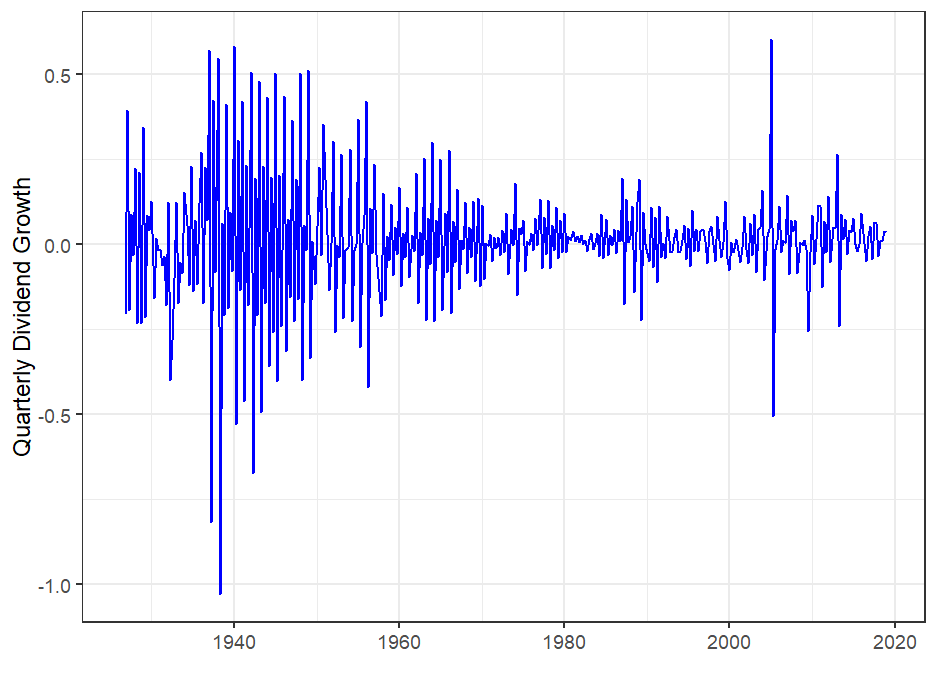
\includegraphics[scale = 0.4]{quarterly_div_growth.png}
	\caption{Quarterly dividend growth: Shows seasonality }
	\label{fig:quarterly_div_growth}
\end{figure}

\begin{figure}[!htb]
	\centering
	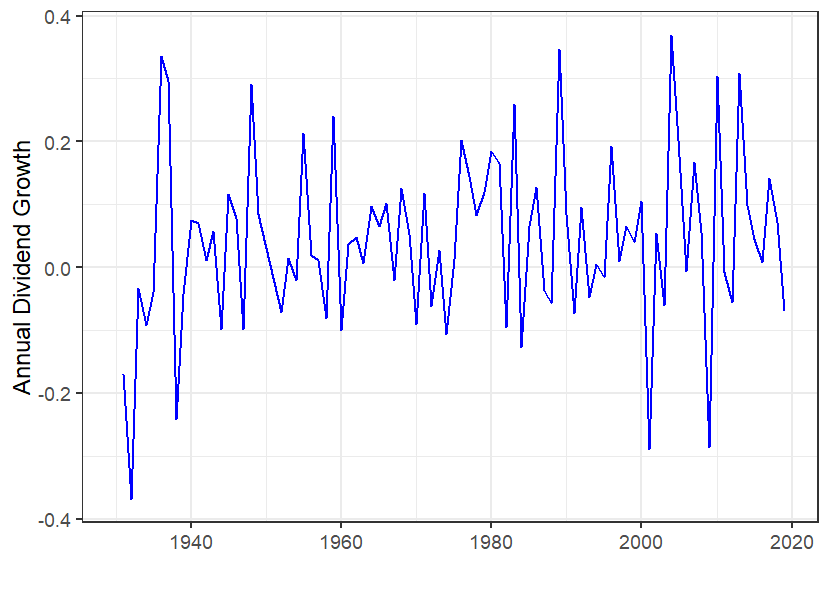
\includegraphics[scale = 0.4]{annual_dividend_growth.png}
	\caption{Annual dividend growth: Smooths out the seasonality issues. Calculated from annual CRSP data on value weighted returns (cum. dividend and ex dividend) }
	\label{fig:annual_div_growth}
\end{figure}
\begin{figure}[!htb]
	\centering
	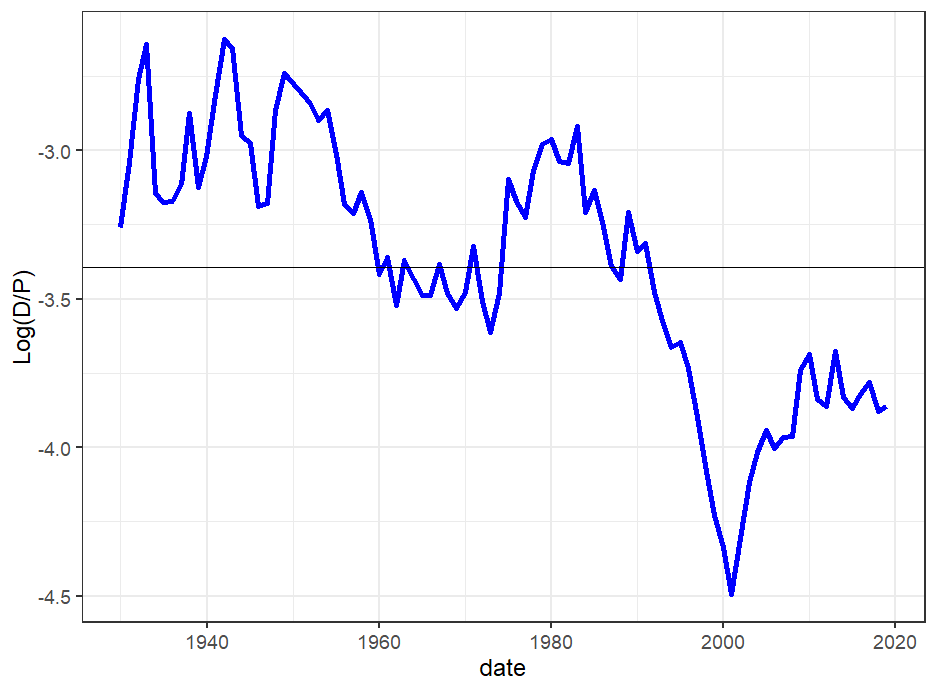
\includegraphics[scale = 0.4]{div_yield_plot.png}
	\caption{Annual dividend yield in logs}
	\label{fig:div_yield}
\end{figure}
\newpage 
\paragraph{d)} Test for a structural break in dividend growth in 1973.2. I run the following regression using demeaned variables  $\Delta d_{t+1} = \alpha + \beta (d_t - p_t) + D (\alpha_D + \beta^D (d_t - p_t))$. The results are reported in Table \ref{table:regressions_structural_break}. The idea is to use a dummy variable for dates past 1973.2 to test whether the relationship between dividend yield and dividend growth in those dates is significantly different from the relationship than before those dates. \\

This is essentially running the test of whether or not coefficients in the following regressions are different. Alternatively, we can run the regressions separately and use an F-test to conduct our statistical inference. 

\begin{equation*}
\begin{split}
 \Delta d_{t+1} &= \alpha + \beta (d_t - p_t) , \text{t less than 1973.2}\\
  \Delta d_{t+1} &= \alpha + \beta (d_t - p_t), \text{t  greater than 1973.2} \\
\end{split}
\end{equation*}
We find that there is significance on the coefficient capturing this effect, $\beta^D$,  indicating there was a structural break in 1973.2.
\begin{table}[!htbp] \centering 
	\caption{Regression of $\Delta d_{t+1} = \alpha + \beta (d_t - p_t) + D (\alpha_D + \beta^D (d_t - p_t))$}
	\label{table:regressions_structural_break} 
	\begin{tabular}{@{\extracolsep{5pt}}lc} 
		\\[-1.8ex]\hline 
		\hline \\[-1.8ex] 
		& \multicolumn{1}{c}{\textit{Dependent variable:}} \\ 
		\cline{2-2} 
		\\[-1.8ex] & dgr\_demean \\ 
		\hline \\[-1.8ex] 
		dp\_demean & 0.249$^{***}$ \\ 
		& (0.042) \\ 
		date\_dummy & 0.070$^{***}$ \\ 
		& (0.022) \\ 
		dp\_demean:date\_dummy & $-$0.223$^{***}$ \\ 
		& (0.052) \\ 
		Constant & $-$0.060$^{***}$ \\ 
		& (0.016) \\ 
		\hline \\[-1.8ex] 
		Observations & 366 \\ 
		R$^{2}$ & 0.090 \\ 
		Adjusted R$^{2}$ & 0.082 \\ 
		Residual Std. Error & 0.179 (df = 362) \\ 
		F Statistic & 11.901$^{***}$ (df = 3; 362) \\ 
		\hline 
		\hline \\[-1.8ex] 
		\textit{Note:}  & \multicolumn{1}{r}{$^{*}$p$<$0.1; $^{**}$p$<$0.05; $^{***}$p$<$0.01} \\ 
	\end{tabular} 
\end{table} 
\quad
\quad 
\quad
\newpage

\section*{Problem 2}
Run a regression of $1, 2, 3, 4, 5, 10$ year returns on log D/P. Are returns forecastable? Contrast different sample period. \\
I run predictive regressions for the samples listed in the tables below and using both quarterly and annual data. Notably, we observe time varying coefficients with the 1947 - 1990 sample generally showing the largest coefficients and t-stats in the annual data sample. When we use quarterly data we see that many of the results hold. The first column of the tables represents the horizon, the second column the estimated coefficient, the third column is the t-stat, and the last column is the r-squared value. 


\begin{table}[!htbp] \centering 
	\caption{Full Sample (left panel uses annual data and right panel uses quarterly)} 
	\label{} 
	\begin{tabular}{@{\extracolsep{5pt}} cccc} 
		\\[-1.8ex]\hline 
		\hline \\[-1.8ex] 
		& b & t(b) & r2 \\ 
		\hline \\[-1.8ex] 
		1 & $0.078$ & $1.611$ & $0.029$ \\ 
		2 & $0.145$ & $2.261$ & $0.050$ \\ 
		3 & $0.211$ & $3.050$ & $0.092$ \\ 
		4 & $0.276$ & $3.843$ & $0.142$ \\ 
		5 & $0.329$ & $5.056$ & $0.173$ \\ 
		10 & $0.567$ & $7.758$ & $0.317$ \\ 
		\hline \\[-1.8ex] 
	\end{tabular} 
\quad
\begin{tabular}{@{\extracolsep{5pt}} cccc} 
	\\[-1.8ex]\hline 
	\hline \\[-1.8ex] 
	& b & t(b) & r2 \\ 
	\hline \\[-1.8ex] 
	1 & $0.015$ & $0.962$ & $0.004$ \\ 
	2 & $0.030$ & $1.530$ & $0.009$ \\ 
	3 & $0.049$ & $2.232$ & $0.015$ \\ 
	4 & $0.073$ & $2.639$ & $0.023$ \\ 
	5 & $0.089$ & $2.919$ & $0.028$ \\ 
	10 & $0.178$ & $5.003$ & $0.060$ \\ 
	\hline \\[-1.8ex] 
\end{tabular} 

\end{table}
\begin{table}[!htbp] \centering 
	\caption{Sample 1926-1990  (left panel uses annual data and right panel uses quarterly)} 
	\label{} 
	\begin{tabular}{@{\extracolsep{5pt}} cccc} 
		\\[-1.8ex]\hline 
		\hline \\[-1.8ex] 
		& b & t(b) & r2 \\ 
		\hline \\[-1.8ex] 
		1 & $0.224$ & $2.580$ & $0.075$ \\ 
		2 & $0.402$ & $3.695$ & $0.119$ \\ 
		3 & $0.538$ & $4.724$ & $0.200$ \\ 
		4 & $0.673$ & $6.111$ & $0.302$ \\ 
		5 & $0.782$ & $7.475$ & $0.353$ \\ 
		10 & $0.937$ & $5.705$ & $0.355$ \\ 
		\hline \\[-1.8ex] 
	\end{tabular} 
\quad \begin{tabular}{@{\extracolsep{5pt}} cccc} 
	\\[-1.8ex]\hline 
	\hline \\[-1.8ex] 
	& b & t(b) & r2 \\ 
	\hline \\[-1.8ex] 
	1 & $0.034$ & $0.913$ & $0.007$ \\ 
	2 & $0.069$ & $1.578$ & $0.016$ \\ 
	3 & $0.115$ & $2.670$ & $0.029$ \\ 
	4 & $0.178$ & $3.099$ & $0.048$ \\ 
	5 & $0.211$ & $3.510$ & $0.056$ \\ 
	10 & $0.409$ & $6.322$ & $0.120$ \\ 
	\hline \\[-1.8ex] 
\end{tabular}
\end{table}

 
\begin{table}[!htbp] \centering 
	\caption{1947 - 1990 Sample  (left panel uses annual data and right panel uses quarterly)} 
	\label{} 
	\begin{tabular}{@{\extracolsep{5pt}} cccc} 
		\\[-1.8ex]\hline 
		\hline \\[-1.8ex] 
		& b & t(b) & r2 \\ 
		\hline \\[-1.8ex] 
		1 & $0.310$ & $3.138$ & $0.204$ \\ 
		2 & $0.487$ & $3.325$ & $0.296$ \\ 
		3 & $0.581$ & $4.291$ & $0.425$ \\ 
		4 & $0.729$ & $7.520$ & $0.544$ \\ 
		5 & $0.991$ & $9.035$ & $0.671$ \\ 
		10 & $1.411$ & $8.417$ & $0.696$ \\ 
		\hline \\[-1.8ex] 
	\end{tabular} 
\quad 
\begin{tabular}{@{\extracolsep{5pt}} cccc} 
	\\[-1.8ex]\hline 
	\hline \\[-1.8ex] 
	& b & t(b) & r2 \\ 
	\hline \\[-1.8ex] 
	1 & $0.057$ & $2.773$ & $0.036$ \\ 
	2 & $0.125$ & $4.131$ & $0.079$ \\ 
	3 & $0.182$ & $5.111$ & $0.114$ \\ 
	4 & $0.249$ & $6.033$ & $0.167$ \\ 
	5 & $0.305$ & $6.518$ & $0.210$ \\ 
	10 & $0.486$ & $9.004$ & $0.393$ \\ 
	\hline \\[-1.8ex] 
\end{tabular} 
\end{table}

\begin{table}[!htbp] \centering 
	\caption{Sample 1947-now  (left panel uses annual data and right panel uses quarterly)} 
	\label{} 
	\begin{tabular}{@{\extracolsep{5pt}} cccc} 
		\\[-1.8ex]\hline 
		\hline \\[-1.8ex] 
		& b & t(b) & r2 \\ 
		\hline \\[-1.8ex] 
		1 & $0.118$ & $2.446$ & $0.083$ \\ 
		2 & $0.203$ & $3.055$ & $0.136$ \\ 
		3 & $0.267$ & $3.852$ & $0.199$ \\ 
		4 & $0.336$ & $5.122$ & $0.252$ \\ 
		5 & $0.431$ & $6.923$ & $0.310$ \\ 
		10 & $0.752$ & $11.933$ & $0.512$ \\ 
		\hline \\[-1.8ex] 
	\end{tabular} 
\quad 
	\begin{tabular}{@{\extracolsep{5pt}} cccc} 
		\\[-1.8ex]\hline 
		\hline \\[-1.8ex] 
		& b & t(b) & r2 \\ 
		\hline \\[-1.8ex] 
		1 & $0.024$ & $2.294$ & $0.018$ \\ 
		2 & $0.051$ & $3.297$ & $0.038$ \\ 
		3 & $0.075$ & $3.918$ & $0.054$ \\ 
		4 & $0.103$ & $4.668$ & $0.077$ \\ 
		5 & $0.129$ & $5.155$ & $0.097$ \\ 
		10 & $0.241$ & $7.220$ & $0.194$ \\ 
		\hline \\[-1.8ex] 
	\end{tabular}
\end{table} 
\begin{table}[!htbp] \centering 
	\caption{1973 - today sample  (left panel uses annual data and right panel uses quarterly)} 
	\label{} 
	\begin{tabular}{@{\extracolsep{5pt}} cccc} 
		\\[-1.8ex]\hline 
		\hline \\[-1.8ex] 
		& b & t(b) & r2 \\ 
		\hline \\[-1.8ex] 
		1 & $0.125$ & $2.254$ & $0.091$ \\ 
		2 & $0.215$ & $2.763$ & $0.170$ \\ 
		3 & $0.299$ & $3.819$ & $0.270$ \\ 
		4 & $0.384$ & $5.260$ & $0.339$ \\ 
		5 & $0.470$ & $6.517$ & $0.405$ \\ 
		10 & $0.876$ & $11.192$ & $0.808$ \\ 
		\hline \\[-1.8ex] 
	\end{tabular} 
\quad 
	\begin{tabular}{@{\extracolsep{5pt}} cccc} 
		\\[-1.8ex]\hline 
		\hline \\[-1.8ex] 
		& b & t(b) & r2 \\ 
		\hline \\[-1.8ex] 
		4 & $0.106$ & $3.856$ & $0.077$ \\ 
		8 & $0.209$ & $5.668$ & $0.169$ \\ 
		12 & $0.300$ & $7.444$ & $0.246$ \\ 
		16 & $0.384$ & $10.076$ & $0.305$ \\ 
		20 & $0.493$ & $13.618$ & $0.402$ \\ 
		40 & $0.944$ & $25.934$ & $0.839$ \\ 
		\hline \\[-1.8ex] 
	\end{tabular}
\end{table} 
\newpage
\section*{Problem 3} Calculate one return at the end of the sample that would bring D/P back to its historical average. \\
I find that a crash of $42.5\%$ brings the dividend yield back to its mean. Including this in our dataset, we see that the point estimates and t-stats all increase by a marginal amount, indicating stronger predictability.   
\begin{table}[!htbp] \centering 
	\caption{Full Sample with crash (annual data)} 
	\label{} 
	\begin{tabular}{@{\extracolsep{5pt}} cccc} 
		\\[-1.8ex]\hline 
		\hline \\[-1.8ex] 
		& b & t(b) & r2 \\ 
		\hline \\[-1.8ex] 
		1 & $0.096$ & $1.894$ & $0.039$ \\ 
		2 & $0.167$ & $2.533$ & $0.062$ \\ 
		3 & $0.228$ & $3.256$ & $0.101$ \\ 
		4 & $0.292$ & $4.047$ & $0.153$ \\ 
		5 & $0.350$ & $5.232$ & $0.186$ \\ 
		10 & $0.577$ & $7.902$ & $0.323$ \\ 
		\hline \\[-1.8ex] 
	\end{tabular} 
\end{table} 

\section*{Problem 4}
Define $X_t = \left[d_t - p_t, d_t - d_{t-1}, r_{ft}\right]'$ where small letters refer to the log of a variable and $r_{ft}$ is the real risk free rate. Run the following VAR.
\begin{equation}
	X_{t+1} = A_0 + A_1 X_t + \epsilon_t
	\label{eq:VAR}
\end{equation}
I get the following estimates for the coefficients, constants, and R-sqaured values. 
\begin{table}[!htbp] \centering 
	\caption{A0 estimates} 
	\label{} 
	\begin{tabular}{@{\extracolsep{5pt}} ccc} 
		\\[-1.8ex]\hline 
		\hline \\[-1.8ex] 
		dp & dgr & rf \\ 
		\hline \\[-1.8ex] 
		-$0.201$ & $0.070$ & $0.004$ \\ 
		\hline \\[-1.8ex] 
     \end{tabular} 
\end{table} 

\begin{table}[!htbp] \centering 
	\caption{A1 coefficient estimates} 
	\label{} 
	\begin{tabular}{@{\extracolsep{5pt}} cccc} 
		\\[-1.8ex]\hline 
		\hline \\[-1.8ex] 
		& dp.l1 & dgr.l1 & rf.l1 \\ 
		\hline \\[-1.8ex] 
		dp & $0.938$ & $$-$0.280$ & $$-$0.706$ \\ 
		dgr & $0.002$ & $$-$0.148$ & $$-$0.675$ \\ 
		rf & $0.001$ & $0.021$ & $0.783$ \\ 
		\hline \\[-1.8ex] 
	\end{tabular} 
\end{table}
\begin{table}[!htbp] \centering 
	\caption{HAC Robust Standard Errors of A0 and A1} 
	\label{} 
	\begin{tabular}{@{\extracolsep{5pt}} cccc} 
		\\[-1.8ex]\hline 
		\hline \\[-1.8ex] 
		$0.125$ & $0.532$ & $0.116$ & $0.005$ \\ 
		$0.037$ & $0.131$ & $0.451$ & $0.017$ \\ 
		$0.134$ & $0.036$ & $0.018$ & $0.052$ \\ 
		\hline \\[-1.8ex] 
	\end{tabular} 
\end{table} 
\begin{table}[!htbp] \centering 
	\caption{R-squared Values} 
	\label{} 
	\begin{tabular}{@{\extracolsep{5pt}} ccc} 
		\\[-1.8ex]\hline 
		 $dp_t$ & $dgr$ & $rf$\\
		\hline \\[-1.8ex] 
		$0.892$ & $0.036$ & $0.585$ \\ 
		\hline \\[-1.8ex] 
	\end{tabular} 
\end{table} 
\paragraph{b)}
The VAR implies little predictability for for dividend growth using the lagged dividend yield. 
\paragraph{c)}
The VAR implies strong predictability of the dividend yield by the lagged dividend yield. Additionally, the R-squared value of this regression if 89.2\%. 
\section*{Problem 5}
\paragraph{a)}Given the VAR approximation above, we can also infer return predictability using the Campbell Shiller approximation:
\begin{equation*}
	r_{t+1} \approx \kappa_0 + \kappa_1 (p_{t+1} - d_{t+1}) - (d_{t+1} - d_t) - (p_t - d_t)
\end{equation*}
To asses the approximation, plot the return implied by the formula with the actual returns from CRSP. In Figure \ref{fig:CS_approx}, we see that this is generally a very accurate approximation. FIgure \ref{fig:CS_error} shows the errors of the approximation over time. Since this is a linearization around the mean, we see that the errors are relatively large when the dividend yield is far away from its historical mean. We find a RMSE of only $0.0043$.

\begin{figure}[!htb]
	\centering
	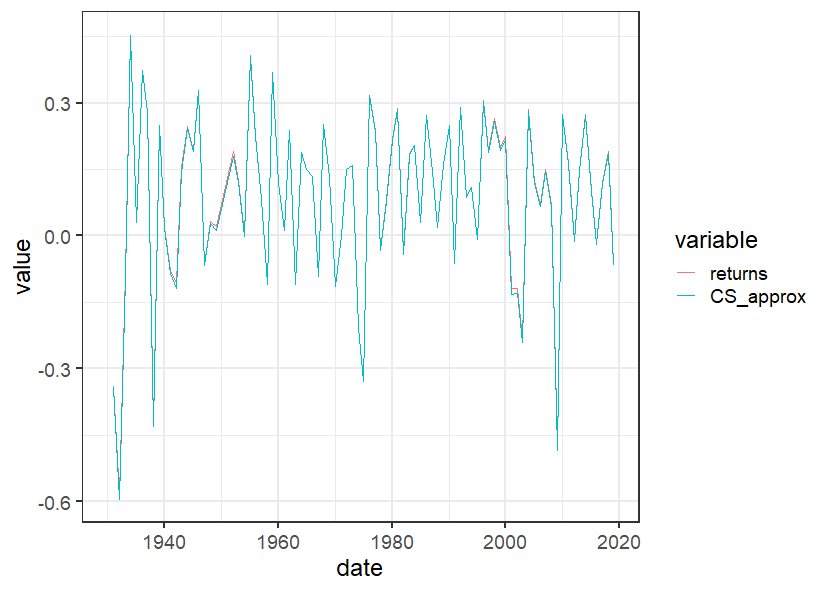
\includegraphics[scale = 0.5]{CS_approx.png}
	\caption{Actual returns vs approximated returns}
	\label{fig:CS_approx}
\end{figure}
\begin{figure}[!htb]
	\centering
	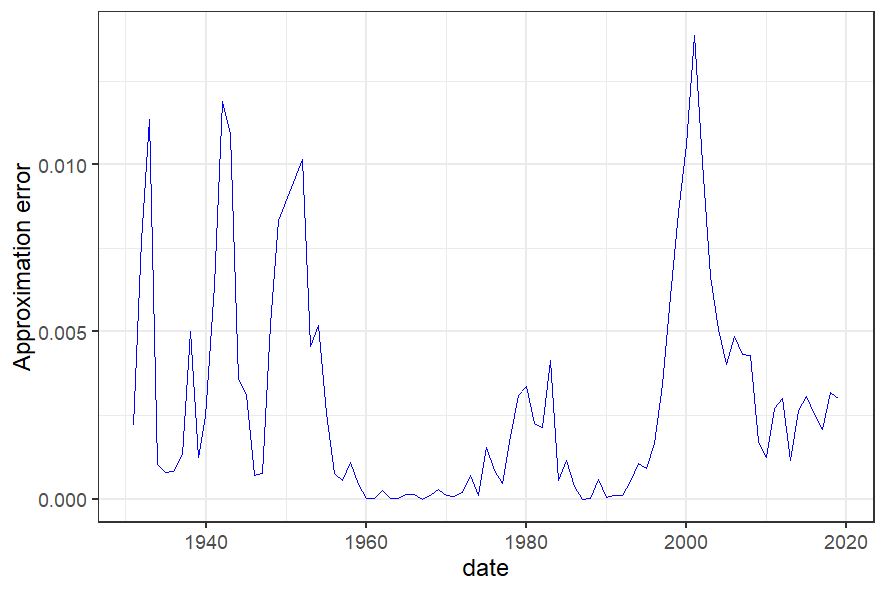
\includegraphics[scale = 0.5]{CS_error.png}
	\caption{Approximation Errors}
	\label{fig:CS_error}
\end{figure}
\paragraph{b)} Now use the above equation and the VAR estimates above to infer the VAR coefficients for predicting the one period ahead return by the dividend yield. Does the dividend yield predict the one period ahead return? Do all three variables predict the one period ahead return?\\


We would like to derive the OLS coefficient for the dividend yield from the VAR and the CS approximation. 
\begin{align*}
\beta_1 &= \frac{Cov(r_{t+1},d_t-p_t)}{Var(d_t-p_t)}
\end{align*}

From the CS-approximation $r_{t+1}=\kappa_0-\kappa_1 (d_{t+1}-p_{t+1}) + (d_t-p_t) + (d_{t+1}-d_t)$, we see that the regression coefficient can be split into terms we know from the VAR
\\
\begin{align*}
\beta_1 &= \frac{Cov((\kappa_0 - \kappa_1 (d_{t+1}-p_{t+1})+ (d_t-p_t) + (d_{t+1}-d_t)),(d_t-p_t))}{Var(d_t-p_t)}\\
&= -\kappa_1 \frac{Cov(d_{t+1}-p_{t+1},d_t-p_t)}{Var(d_t-p_t)} +\frac{Cov(d_{t+1}-d_{t},d_t-p_t)}{Var(d_t-p_t)}+1\\
&= -\kappa_1 A^1_{1,1} + A^1_{2,1} + 1\\
\end{align*}

Where $A^1_{1,1}$ and $A^1_{2,1}$ denote the coefficients from equation (\ref{eq:VAR}). With $\kappa_1=0.967$, we get the following estimate

\begin{align*}
\beta_1 &= -0.967 * 0.938 + (0.002) + 1 = 0.0947\\
\end{align*}

Standard errors can be inferred using the delta method. Generally,

\begin{align*}
Var(P(X A_1)) &= Var( \frac{\partial P(X_i A_1)}{X A_1} X A_1) = (\frac{\partial P(X_i A_1)}{X A_1})' V (\frac{\partial P(X_i A_1)}{X A_1})
\end{align*}

Where the first (sandwich) term is the Jacobian (i.e. vector of first-order partial derivatives of the inverse link function), and the middle term $V=Var(X\beta)$ is the variance-covariance matrix of the estimators from the original VAR(1) model.  

\begin{align*}
\hat{SE(\beta_1)}=0.038
\end{align*}

Similarly, the $R^2$:

\begin{align*}
R^2_1=0.0358
\end{align*}

We are able to reject the null of $\beta_1=0$ at a five percent significance level, but the $R^2$ is only $4.2\%$. Thus, we find for predictability of one period ahead returns based on dividend yields.  

The regression we are interested in estimating for predicting one period head returns based on all three of our variables is
\begin{align*}
r_{t+1} &= \beta_0 +  \beta_1 (d_t-p_t) + \beta_2 (d_t-d_{t-1}) + \beta_3 r_{ft} \epsilon_{t+1}\\
\end{align*}

Thus, the coefficients we would like to derive from the VAR and CS approximation are given by
\begin{align*}
\beta_1 &= \frac{Cov(r_{t+1},d_t-p_t)}{Var(d_t-p_t)}\\
\beta_2 &= \frac{Cov(r_{t+1},d_t-d_{t-1})}{Var(d_t-d_{t-1})}\\
\beta_3 &= \frac{Cov(r_{t+1},r_{ft})}{Var(r_{ft})}\\
\end{align*}

Using the same strategy as above, we get the following
\begin{align*}
\boldsymbol{\beta_{d_t-p_t}} &= \frac{Cov((\kappa_0 - \kappa_1 (d_{t+1}-p_{t+1})+ (d_t-p_t) + (d_{t+1}-d_t)),(d_t-p_t))}{Var(d_t-p_t)}\\
&= -\kappa_1 \frac{Cov(d_{t+1}-p_{t+1},d_t-p_t)}{Var(d_t-p_t)} +\frac{Cov(d_{t+1}-d_{t},d_t-p_t)}{Var(d_t-p_t)}+1\\
&= -\kappa_1 A^1_{1,1} + A^1_{2,1} + 1\\
\end{align*}

\begin{align*}
\boldsymbol{\beta_{d_t - d_{t-1}}} &= \frac{Cov(\kappa_0 - \kappa_1 (d_{t+1}-p_{t+1})+ (d_t-p_t) + (d_{t+1}-d_t),d_{t}-d_{t-1})}{(d_{t}-d_{t-1})}\\
&= -\kappa_1 \frac{Cov(d_{t+1}-p_{t+1},d_{t}-d_{t-1})}{Var(d_{t}-d_{t-1})} +\frac{Cov(d_{t}-p_{t},d_{t}-d_{t-1})}{Var(d_{t}-d_{t-1})}\\ &+\frac{Cov(d_{t+1}-d_{t},d_{t}-d_{t-1})}{Var(d_{t}-d_{t-1})}\\
&= -\kappa_1 A^1_{2,3} + 0 + A^1_{2,2}\\
\end{align*}

\begin{align*}
\boldsymbol{\beta_{r_ft}} &= \frac{Cov(\kappa_0 - \kappa_1 (d_{t+1}-p_{t+1})+ (d_t-p_t) + (d_{t+1}-d_t)),r_{ft})}{r_{ft}}\\
&= -\kappa_1 \frac{Cov(d_{t+1}-p_{t+1},r_{ft})}{Var(r_{ft})} +\frac{Cov(d_{t}-p_{t},r_{ft})}{Var(r_{ft})}\\ &+\frac{Cov(d_{t+1}-d_{t},r_{ft})}{Var(r_{ft})}\\
&= -\kappa_1 A^1_{1,3} + 0 + A^1_{2,3}\\
\end{align*}

$\frac{Cov(d_{t}-p_{t},(d_{t+1}-d_t))}{Var(d_{t+1}-d_t)}$ and $\frac{Cov(d_{t}-p_{t},r_{ft})}{Var(r_{ft})}=0$ as the VAR(1)-specification does not provide for contemporary correlation between the regressors (e.g. implicitly restricts these coefficients to be zero). \\

\begin{align*}
\beta_{d_t-p_t} &= -0.967 * 0.938 + (0.002) + 1 = 0.0947\\
\beta_{d_t - d_{t-1}} &=  0.504\\
\beta_{r_ft} &= 0.008\\
\end{align*}

Standard errors are	

\begin{align*}
\hat{SE(\beta_{d_t-p_t})}=0.038\\
\hat{SE(\beta_{d_t - d_{t-1}})}=0.168\\
\hat{SE(\beta_{r_ft})}=0.425\\
\end{align*}

The implied coefficient estimate on dividend yield is significant, dividend yield is significant, and real risk-free rates are insignificant at the 5\% significance level. Based on a F-test of joint significance, we fail to reject the Null of no joint predictability of one-period ahead returns.



\section*{Problem 6}
\paragraph{a)}Report direct return regression results and compare them to the VAR implied results for horizons of 1, 3, and 5 years. \\

We first run two regressions separately of the form shown in Equation \ref{eq:direct_regressions} to obtain the direct regression coefficients shown in Table \ref{table:div_yield_regressions}. 
\begin{equation}
	\begin{split}
	r_{t, t+\tau} & = \alpha_r + \beta_{r, \tau}(d_t - p_t) + \epsilon^r_{t+\tau}\\
	\Delta d_{t, t+\tau} & = \alpha_{\Delta_d}+\beta_{\Delta d, \tau}(d_t - p_t)+ \epsilon^dp_{t+\tau}\\
	\end{split}
	\label{eq:direct_regressions}
\end{equation}
the results of which are shown in Table (\ref{table:div_yield_regressions}). The results suggest all variation in market price-dividend ratios corresponds to changes in expected variation in risk premiums and none about news to future dividend growth.\footnote{ Recall, we can decompose the log price dividend ratio, denoted as $z_t$ here, as
\begin{equation*}
	Var(z_t) = \sum_{j=0}^{\infty}\kappa^j_1\left[Cov(g_{t+1+j}, z_t)- Cov(r_{t+1+j}, z_t)\right]
\end{equation*}
Thus, if both returns and dividends are unforecastable, the price divdend ratio should be constant, which it clearly is not in Figure \ref{fig:div_yield}. We cannot ask "are returns forecastable?", rather we must ask "which of dividend growth or returns are forecastable?" A null hypothesis that specifies returns are not forecastable must also that dividend growth is forecastable. That is we need to test the joint distribution of return and dividend-growth forecastability. } We also see that the point estimates for $\beta_{r, \tau}$ are increasing with horizon. 




Next, we calculate the implied regression coefficients from our VAR and the Campbell Shiller linearization of a return
\begin{equation*}
	r_{t+1} \approx \rho + \kappa(p_{t+1} - d_{t+1}) + (d_{t+1}-d_t) - (p_t - d_t)
\end{equation*}

\noindent The implied coefficient on returns is given by
\begin{equation*}
	\beta_{r, \tau} = \frac{Cov(r_{t, t+\tau}, e_{1}'X_t)}{Var(e_{1}'X_t)}
\end{equation*}
We can solve for $r_{t+k}$ as follows
\begin{equation}
\begin{split}
	r_{t+k} &= [-\kappa\quad 1 \quad 0] \left(X_{t+k}\right) + e_1 (X_{t + k -1})\\
	&= [-\kappa\quad 1 \quad 0] \left(A(X_{t+k-1}) + \epsilon_{t+k} \right) + e_1 (X_{t+k-1})\\
	& = ([-\kappa\quad 1 \quad 0]A + e_1) X_{t+k-1} + [-\kappa\quad 1 \quad 0]\epsilon_{t+k}\\
	& =([-\kappa\quad 1 \quad 0]A + e_1) A^{k-1} X_t  + ([-\kappa\quad 1 \quad 0]A + e_1)\sum_{j = 0}^{k-2} A^j\epsilon_{t+k-j} +[-\kappa\quad 1 \quad 0]\epsilon_{t+k} \\
\end{split}
\label{eq:VAR_implied_r}
\end{equation}
where the last equality holds by backwards iteration and using our VAR.  Thus, we can derive $r_{t, t+\tau}$ as
\begin{equation*}
\begin{split}
r_{t, t+\tau}  &= \sum_{k = 1}^{\tau} r_{t+k}\\
& = \sum_{k = 1}^{\tau}\bigg(([-\kappa\quad 1 \quad 0]A + e_1) A^{k-1} X_t  + ([-\kappa\quad 1 \quad 0]A + e_1)\sum_{j = 0}^{k-2} A^j\epsilon_{t+k-j} +[-\kappa\quad 1 \quad 0]\epsilon_{t+k} \bigg)\\
& =  \sum_{k = 1}^{\tau}(([-\kappa\quad 1 \quad 0]A + e_1) A^{k-1} X_t) + \sum_{k = 1}^{\tau}\sum_{j = 0}^{k-2}( [-\kappa\quad 1 \quad 0]A + e_1) A^j\epsilon_{t+k-j} +[-\kappa\quad 1 \quad 0]\epsilon_{t+k}\\
\end{split}	
\end{equation*}

Using equation (\ref{eq:VAR_implied_r}), we solve for our coefficient of interest as follows 

\begin{equation*}
	\begin{split}
     \beta_{r, \tau} &= \frac{Cov(r_{t, t+\tau}, e_{1}'X)}{Var(e_{1}'X)}\\
     &= \frac{Cov(\sum_{k = 1}^{\tau}([-\kappa\quad 1 \quad 0]A + e_1) A^{k-1} X_t), e_{1}'X)}{Var(e_{1}'X)}\\
     &= ([-\kappa\quad 1 \quad 0]A + e_1)\sum_{k = 1}^{\tau}A^{k-1}\bigg(\frac{Var(X_t)e_{1}}{e_{1}'Var(X)e_1}\bigg)
	\end{split}
\end{equation*}
R-squared is then given by
\begin{equation*}
	R^2 = \frac{Cov(r_{t, t+\tau}, e_{1}'X)^2}{Var(r_{t, t+ \tau})Var(e_1'X)} =\beta^2_{r, \tau}\frac{Var(e_1'X)}{Var(r_{t, t+\tau)}}
\end{equation*}
We can directly infer dividend growth from the VAR
\begin{equation*}
\begin{split}
	X_{t+k} = A^k X_t + \sum_{j=0}^{k=1}A^j \epsilon_{t+k-j}\\
	e_2'X_{t+k} = e_2'A^kX_t + e_2'\sum_{j = 0}^{k-1}A^j \epsilon_{t+k-j}
\end{split}
\end{equation*}
Therefore $\Delta d_\tau = \sum_{k=0}^\tau e_2' X_{t+k} = e_2'\sum_{k=1}^{\tau}A^kX_t + \sum_{k=1}^{\tau}e_2'\sum_{j = 0}^{k-1}A^j \epsilon_{t+k-j}$, which implies our regression coefficient is
\begin{equation*}
	\begin{split}
		\beta_{\Delta d, \tau} &= \frac{Cov(\Delta d_{t + \tau}, e_{1}'X)}{Var(e_{1}'X)}\\
		& = \frac{Cov(e_2' A^k X, e_{1}'X)}{Var(e_{1}'X)}\\
		& = \frac{e_2' (\sum_{k=1}^{\tau}A^k)var(X_t)e_1}{e_1'Var(X_t)e_1}
	\end{split}
\end{equation*}
Therefore the $R^2$ is given by 

\begin{equation*}
R^2 = \frac{Cov( \Delta d_{t+\tau}, e_{1}'X)^2}{ Var(\Delta d_{t+\tau})Var(e_1'X)} =\beta^2_{ \Delta d_{t+\tau},}\frac{Var(e_1'X)}{Var( \Delta d_{t+\tau})}
\end{equation*}	
The comparison of the implied and direct coefficients is shown in Table \ref{table:div_yield_regressions}
\begin{table}[!htbp] \centering 
	\label{} 
	\begin{tabular}{@{\extracolsep{5pt}} c|ccc|cc} 
		\\[-1.8ex]\hline 
		\hline \\[-1.8ex] 
	Horizon (Years)	& OLS $\beta_{r, \tau}$ & t($\beta_{r, \tau}$) & $R^2$ & VAR implied $\beta_{r, \tau}$ & VAR implied $R^2$ \\ 
		\hline \\[-1.8ex] 
		1 & $0.078$ & $1.611$ & $0.029$ & $0.079$ & $0.030$ \\ 
		3 & $0.211$ & $3.050$ & $0.092$ & $0.223$ & $0.104$ \\ 
		5 & $0.329$ & $5.056$ & $0.173$ & $0.351$ & $0.200$ \\ 
		\hline \\[-1.8ex] 
	\end{tabular} 
	\quad
	\begin{tabular}{@{\extracolsep{5pt}} c|ccc|cc} 
		\\[-1.8ex]\hline 
		\hline \\[-1.8ex] 
	Horizon(Years)	& OLS $\beta_{\Delta d, \tau}$ & t($\beta_{\Delta d, \tau}$) & $R^2$ & VAR implied $\beta_{\Delta d, \tau}$ & VAR implied $R^2$ \\ 
		\hline \\[-1.8ex] 
	1 & $0.005$ & $0.135$ & $0.0003$ & -$0.010$ & $0.001$ \\ 
	3 & $-0.012$ & -$0.201$ & $0.001$ & -$0.010$ & $0.0004$ \\ 
	5 & $-0.005$ & -$0.072$ & $0.0001$ & -$0.010$ & $0.0003$ \\ 
		\hline \\[-1.8ex] 
	\end{tabular}
	\caption{Return regressions (top panel) and dividend growth regressions (bottom panel)} 
	\label{table:div_yield_regressions}
\end{table} 
\paragraph{b)} Can you infer how much of the variation of the price dividend ration is due to variation in cashflows and how much is due to variation in future returns, at each of these horizons?\\

We consider the following decomposition of price dividend ration variance, assuming $p-d$ is stationary
\begin{equation}
	1 = \frac{Cov(\sum_{j=0}^{\infty})\kappa_1^jg_{t+1+j}, z_t}{Var(z_t)} - \frac{Cov(\sum_{j=0}^{\infty})\kappa_1^jr_{t+1+j}, z_t}{Var(z_t)}
	\label{eq:variance_decomposition}
\end{equation} 
Equation (\ref{eq:variance_decomposition}) gives the contribution of dividend growth and returns to the variance of the price dividend ratio in the form of regression coefficients. Thus, we can consider the following projections

\begin{equation*}
\begin{split}
	\sum_{j=0}^{J} \kappa_1^j g_{t+1+j} &= \beta_{0, g} + \beta_g z_t +u_{g, t+J}\\
	\sum_{j=0}^{J} \kappa_1^j g_{t+1+j} &= \beta_{0, r} + \beta_r z_t +u_{r, t+J}\\
\end{split}
\end{equation*}
which imply we can calculate $\beta_g = \sum_{j=0}^{J}\kappa_1^j\beta_{g, j}$ and $\beta_r = \sum_{j=0}^{J}\kappa_1^j \beta_{r, j}$ to calculate the percentage of the variance of $z$ explained by future future growth rates of dividends and that explained by future returns. The return contribution is $-54\%$ and the dividend contribution is about $-8.3 \%$.

\section*{Problem 7}
Plot the response of this system to dividend growth and dividend yield shocks. Plot the response of the level of dividends, not their growth rate. Include responses of returns are prices to your shocks. \\

See figures \ref{fig:impulse_responses} and \ref{fig:price_and_return_irfs}. To calculate the responses of prices and returns, we use the following iterations
\begin{itemize}
	\item Define initial prices to be 1
	\item Exponentiate our responses of dividend yield and dividend growth to get prices and dividends in levels rather than logs
	\item Use the initial or previous value of dividend to calculate the current dividend based off of the exponentiated value of dividend growth
	\item Use our updated value of the dividend and the current price dividend ratio to update our price
	\item repeat until we have calculated the the entire response funtion
\end{itemize}
Since we are defining initial prices at a certain level, only the shape of the responses not the level can be interpreted. 
 
\begin{figure}[!htb]
	\centering
	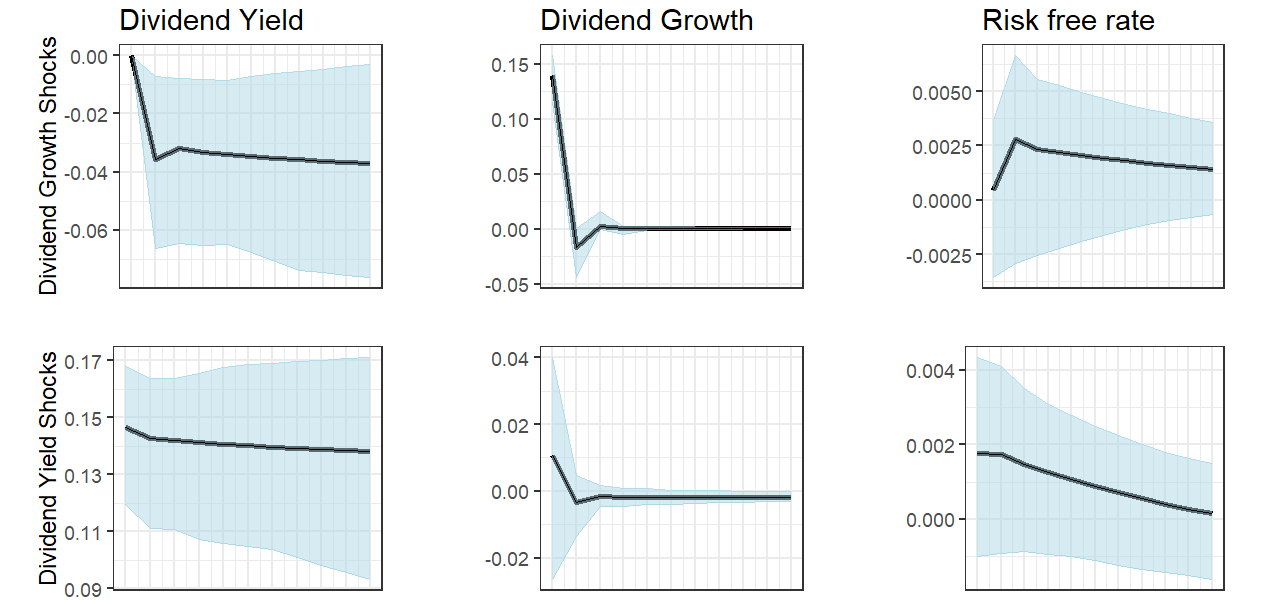
\includegraphics[scale = 0.5]{irfs.png}
	\caption{Impulse responses to dividend growth (top row) and dividend yield (bottom row) shocks. Columns represent the responses of dividend yields, dividend, growth, and risk free rates respectively. }
	\label{fig:impulse_responses}
\end{figure}

\begin{figure}[!htb]
	\centering
	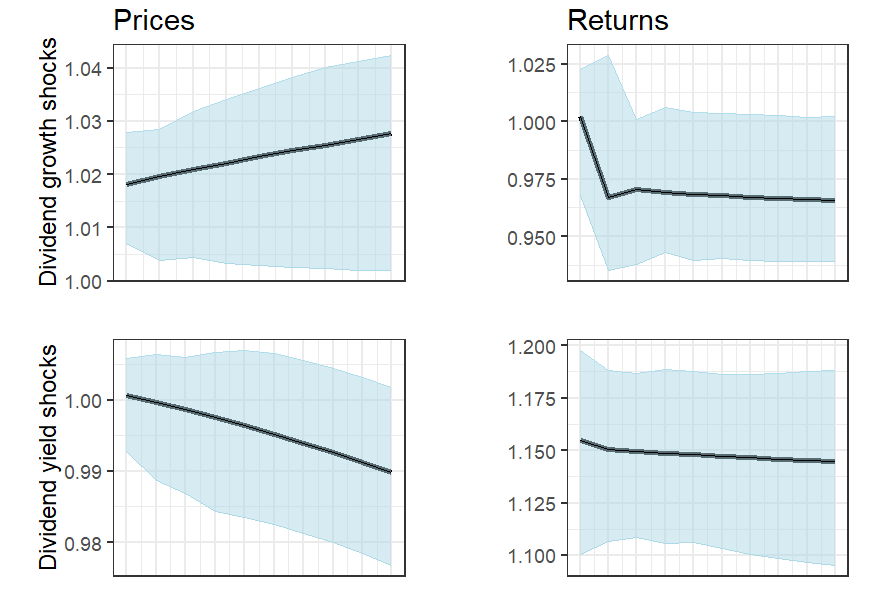
\includegraphics[scale = 0.5]{price_and_return_irfs.png}
	\caption{Impulse responses of prices and returns to dividend growth (top row) and dividend yield (bottom row) shocks. }
	\label{fig:price_and_return_irfs}
\end{figure}
\section*{Problem 8}
\paragraph{a)} Looking now at the shape of the responses, can we still label one shock an expected return shock and the other a cashflow shock? \\

No. The two shocks in Figure \ref{fig:impulse_responses} look like they are essentially the same shock. 

\paragraph{b)}
Let $\epsilon_{r,t}$ be the shock to the return forecasted by
$d_t - p_t$, which you can again approximate by
$\epsilon_{r,t} = \kappa \epsilon_{1,t} - \epsilon_{2,t}$.
How correlated are the shocks $\epsilon_{1,t}$, $\epsilon_{r,t}$,
and $\epsilon_{2,t}$? Does the fact that the $\epsilon_{1,t}$
and $\epsilon_{2,t}$ correlation is not exactly zero matter to the imulse response interpretation? 

Taking the fitted residuals from the VAR system given in Question 4,
we can construct the $\epsilon_{r,t}$ series as asked. Taking the
sample correlation gives us the following correlation matrix:

\begin{table}[!htbp] \centering 
	\label{} 
	\begin{tabular}{@{\extracolsep{5pt}} c|ccc} 
		
		& $\epsilon_{1,t}$ & $\epsilon_{2,t}$ & $\epsilon_{r,t}$ \\
		\hline \\[-1.8ex] 
		$\epsilon_{1,t}$ & $1$ & $0.007$ & $0.996$ \\ 
		$\epsilon_{2,t}$ & $0.007$ & $1$ & $-0.081$ \\ 
		$\epsilon_{r,t}$ & $0.996$ & $-0.081$ & $1$ \\ 
		\hline
	\end{tabular} 
	\caption{Correlation of Shocks} 
\end{table} 

Reading from the sample correlation matrix,
the shocks are either extremely correlated
(e.g. 0.996 for $\epsilon_{1,t}$ and $\epsilon_{r,t}$)
or almost uncorrelated. As pointed out in the problem,
$\epsilon_{1,t}$ and $\epsilon_{2,t}$ correlation is
not exactly zero; however, it is very small, at about
0.007.

\paragraph{c)}

Usually, the first assumption made in interpreting impulse
response functions is that the shocks should be orthogonal.
The IRF asks the question "what happens to $y_{i,t+k}$ if $\epsilon_{j,t}$ has a unit impulse, leaving $\epsilon_{i,t}$
fixed for $i\neq j$?"; however, in the case when the shocks themselves
are correlated, this question is somewhat ill-posed.

Say we have some VAR with

$$
X_{t+1}  = AX_t + \epsilon_{t+1}
$$
where 
$$
\mathbb{E} [\epsilon_t \epsilon_t^{\prime}]  = \Omega
$$

Then we can take the Cholesky factor, $S$, of the matrix
$\Omega$, which is the unique lower triangular matrix such that
$SS^\prime = \Omega $. Furthermore, define the orthogonal shocks
$\eta_t = S^{-1}\epsilon_t$, so that we can rewrite the VAR as

$$
X_t = C(L)S\eta_t
$$

where C(L) is the (inverted) lag polynomial. This gets us to

\begin{equation*}
%\begin{split}
%\mathbb{E}[\eta_t \eta_t^{\prime}] &= \mathbb{E}[S^{-1}\epsilon_t \epsilon_t^{\prime}S^{-1}^\prime] \\
%&= S^{-1}\mathbb{E}[\epsilon_t \epsilon_t^{\prime}]S^{-1}^\prime \\
%&= S^{-1} \Omega S^{-1}^\prime \\
%&= S^{-1} SS^{\prime} S^{-1}^\prime \\
%&= I\\
%\end{split}
\end{equation*}

More broadly, we can define for any orthogonal matrix $H$,
$w_t = (SH)^{-1}\epsilon_t$, from which we can recover
the general class of orthonormal representation of $X_t$:

\begin{equation*}
\begin{split}
X_t & = C(L)S\eta_t \\
& = F(L) w_t
\end{split}
\end{equation*}

The issue is then choosing (in the sense of identification) the
matrix $H$. If the non-diagonal terms in the VAR coefficient matrix
are zero, then this question is more straightforward. Orthogonalize
the shocks via Cholesky (or Spectral) Decomposition, and the
right hand side shocks can be interpreted as an
expected return shock, a cashflow shock, and so on and so forth. \\

If we do not have such restrictions, however, we have to rely on
economic theory to give us such restrictions. Given an $n$-dimensional
VAR (demeaned), then we have $n^2$ parameters to pin down.
$n(n+1)/2$ parameters can be found by the orthonormality
restrictions, but we still need to figure out the other
free parameters, $n(n-1)/2$ of them. For example,
the theory may tell us that the second shock does not affect
the dividend yield in the long run; or that the sign of
the interaction must be negative, etc. While in some cases,
the identification may not be exact, this helps us make progress
in the right direction.

\paragraph{d)}

Run a restricted VAR with just return and the dividend yield. The impulse responses of this system are shown in Figure \ref{fig:restrictred_VAR}.
Since the impulse response from dp shock
is very close to zero, it is similar to the $a_{12}=0$
initially mentioned in part (c) above. 

\begin{figure}[!htb]
	\centering
	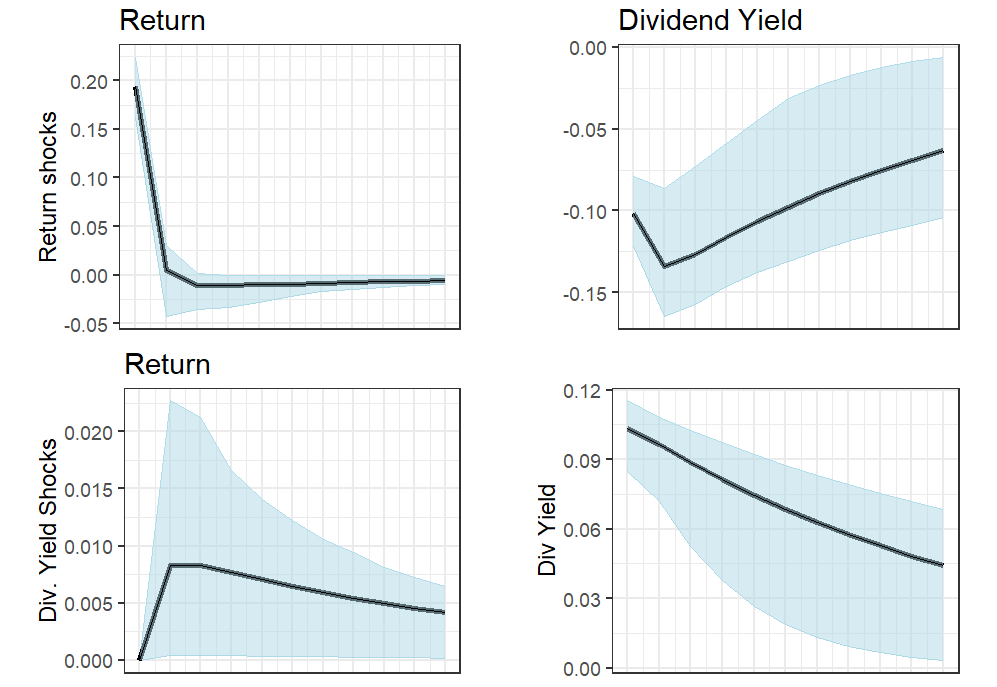
\includegraphics[scale = 0.5]{restircted_var_shock.png}
	\caption{Impulse response function from the restricted VAR}
	\label{fig:restrictred_VAR}
\end{figure}

\paragraph{e)}


Taking our estimate of restricted VAR composed of return and
dividend yield from d) as the null model, we bootstrap the VAR.
This is done by drawing residuals (with replacement) from
the empirical distribution, fitting the VAR each time,
and saving the estimated coefficient in each iteration.


According to this exercise, the median of the estimated
coefficient is at around 0.035, which is nearly
half of OLS estimate of 0.078, suggesting an upward
bias in the OLS estimate. Note that the OLS estimator, while
consistent, is biased in small samples. On the other hand, at
least from this exercise, it is not clear how "wrong" the standard errors are. However, from our lecture notes, we see that
the OLS setting may yield slightly smaller
standard errors than what may be computed from "true" properties.
The depressed standard errors lead to
inflated t statistics, inducing us
to (perhaps falsely) reject of the null hypothesis of
$\hat{\beta}=0$. 

\begin{figure}[!htb]
	\centering
	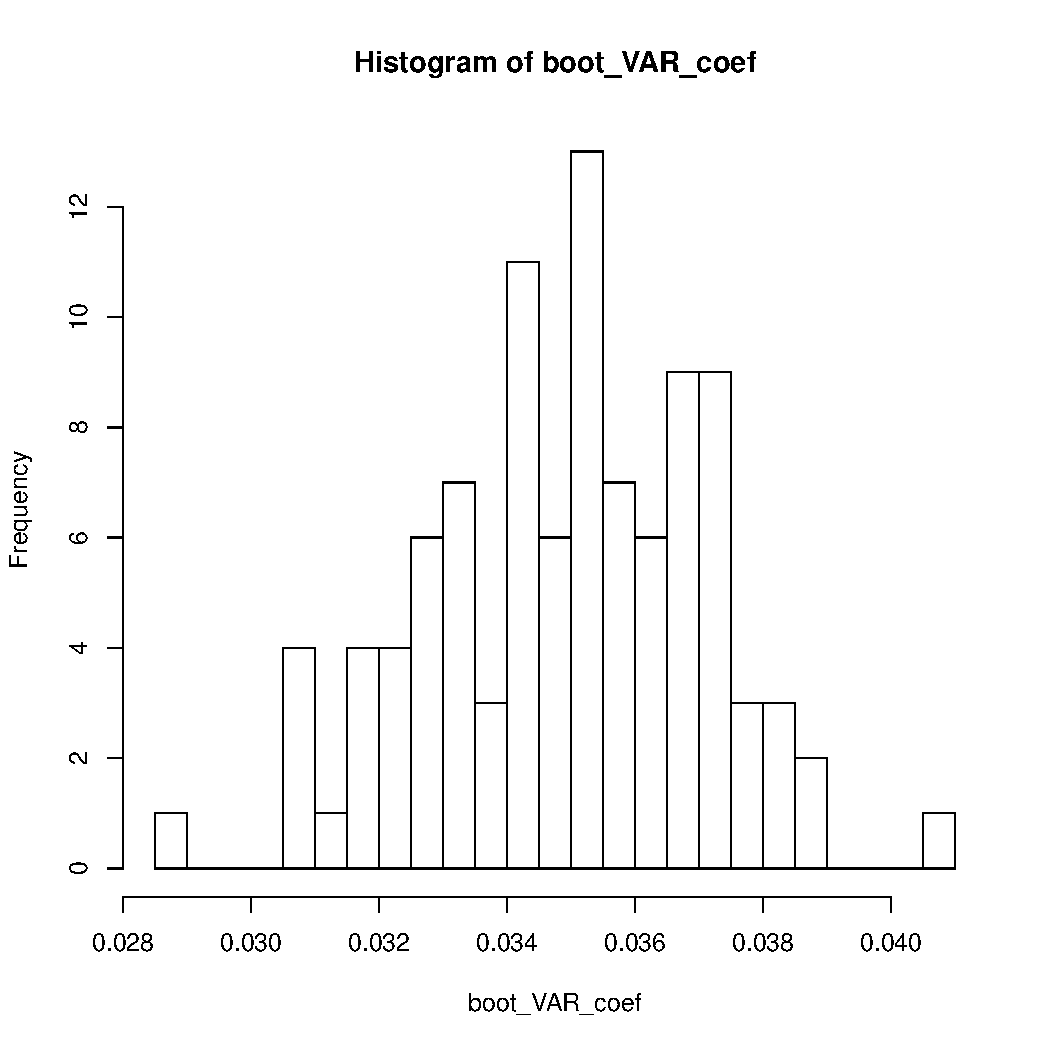
\includegraphics[scale = 0.5]{boot_VAR_coef.pdf}
	\caption{Bootstrapped coefficients of one year log returns on lagged D/P. Sample size = 1000, Number of samples = 100}
	\label{fig:boot_VAR_coef}
\end{figure}

% ================================================================
% Problem 9
% ================================================================
\section*{Problem 9}
Our VAR and CS decomposition together imply the following holds
\begin{equation}
	e_1' = e_2'A\left[I - \kappa_1A\right]^{-1} - e_3'A\left[I - \kappa_1 A\right]^{-1}
\end{equation}
Using the VAR approach we can estimate each piece to get the return news decompostion as follows
\begin{equation*}
	r_t - E_{t-1}\left[r_t\right] = e_2'A\left[I - \kappa_1A\right]^{-1}u_t - e_3'A\left[I - \kappa_1 A\right]^{-1}u_t
\end{equation*}
where $u_t$ is the vector of VAR innovations. The result is shown in Figure \ref{fig:news_decomposition}.
\begin{figure}[!htb]
	\centering
	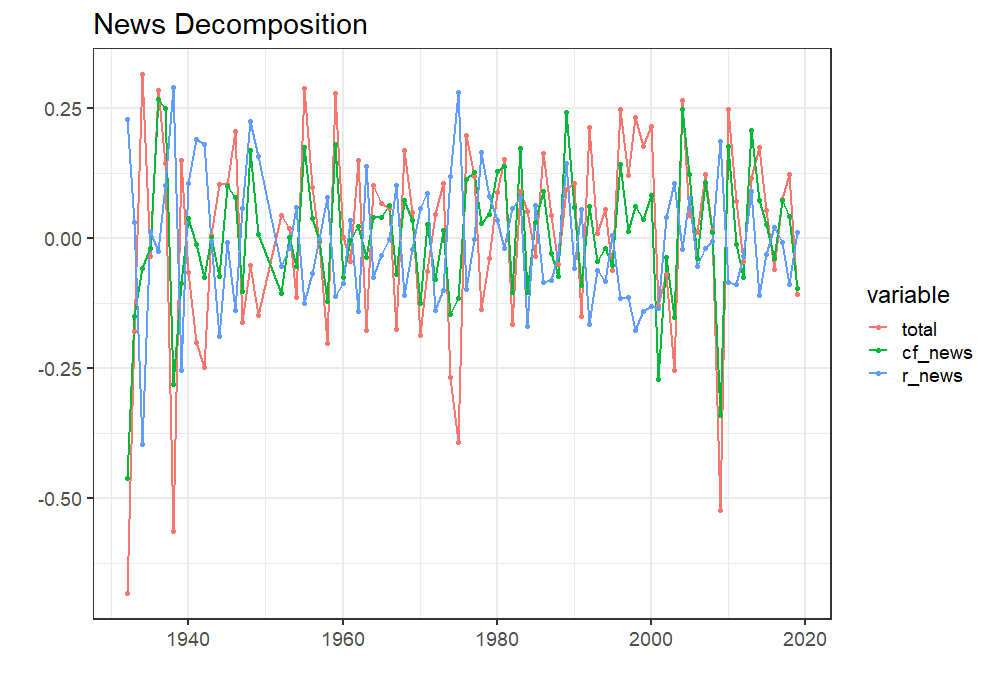
\includegraphics[scale = 0.5]{news_decomposition.png}
	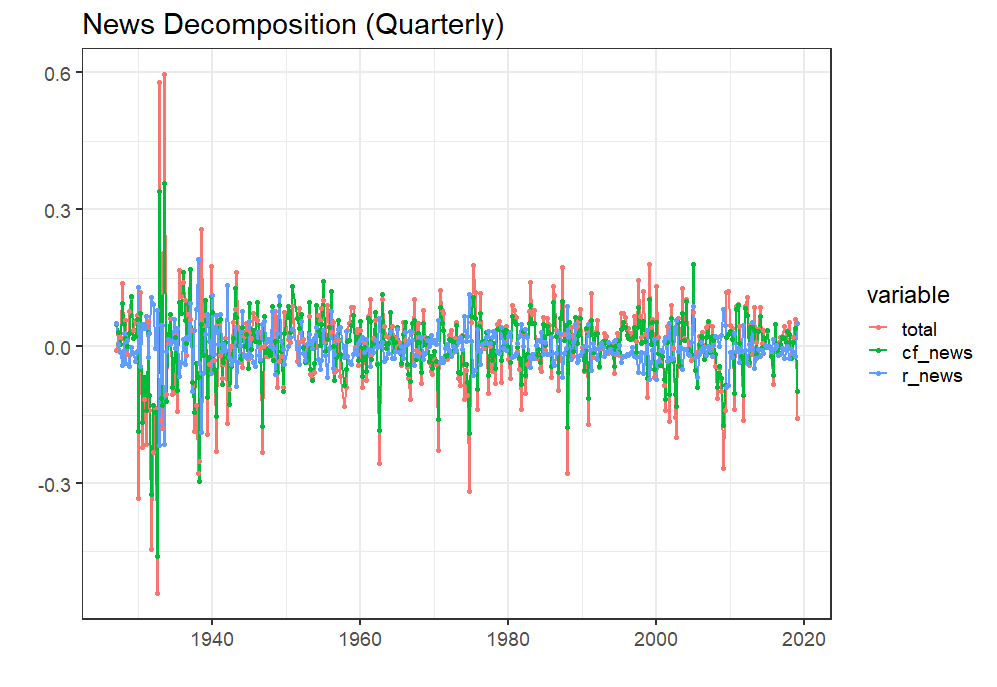
\includegraphics[scale = 0.5]{news_decomp_qrtly.png}
	\caption{News Decomposition annual and quarterly}
	\label{fig:news_decomposition}
\end{figure}

The average absolute error for the 
approximate identity  is
0.007687201. 
% ================================================================
% Problem 10
% ================================================================
\section*{Problem 10}
Compute and plot the graphs of 
\begin{align*}
r_{t}   =E_{t-1}r_{t} + (E_{t}-E_{t-1}) \left[ \Delta d_{t+j} + \sum^\infty_{j=1} \kappa^{j-1} \Delta d_{t+j} - \sum^\infty_{j=1} \kappa^{j-1} r_{t+j}\right]\\
\end{align*}
Variables are demeaned prior to estimating the previously specified VAR(1). The individual elements of the decomposition are 
\begin{equation*}
	\begin{split}
	 E_{t-1}(r_t) &= [\kappa,\ 1,\ 0]'A_1X_{t-1}-e_1'X_{t-1}\\
	  E_{t-1}\Delta d_t &= e_2'A_1X_{t-1}\\
	  E_{t-j}\sum^\infty_{j=1}\kappa^{j-1}\Delta d_{t+j} &= e_2' A_1(I_3-kA_1)^{-1}X_{t-j}\\
	  E_{t-j}\sum^\infty_{j=1}\kappa^{j-1}r_{t+j} &= \left[ [\kappa,\ 1,\ 0]' (I_3 - \kappa A_1)^{-1} -e_1' ( I_3 -\kappa A_1)^{-1} \right]X_{t-j}
	\end{split}
\end{equation*}


where $j is$ is 0 or 1 and the elementary vectors are as described before. 

Comparing Figure \ref{fig:news_decomposition_returns} and Figure \ref{fig:news_decomposition}, we see that the news decompositions are approximately the same. 

\begin{figure}[!htb]
	\centering
	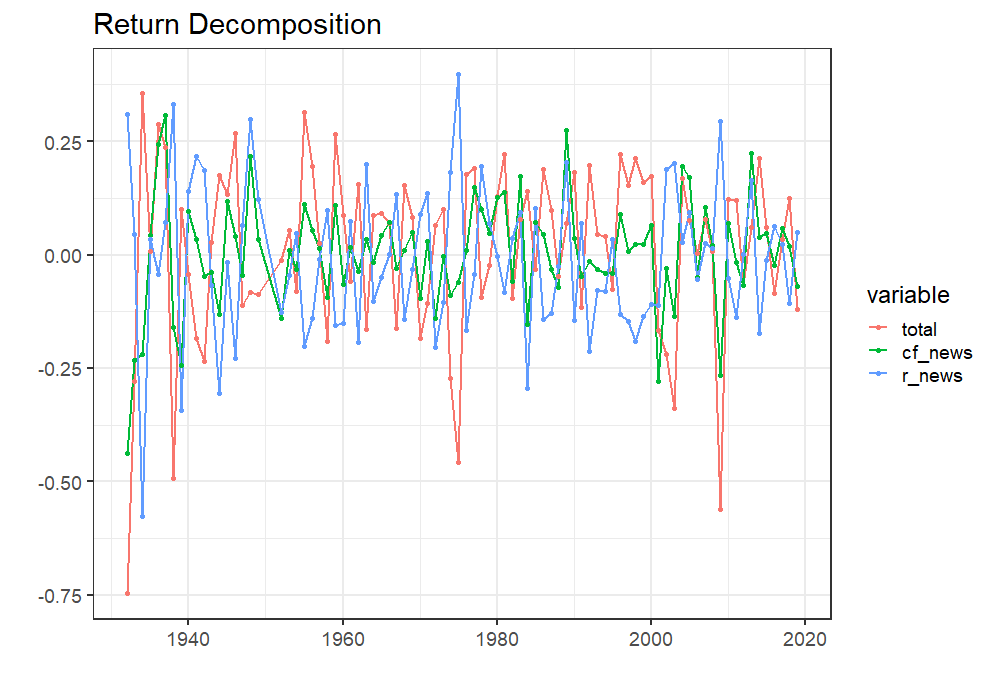
\includegraphics[scale = 0.5]{return_decomposition_returns.png}
	\caption{News Decomposition using return decomposition}
	\label{fig:news_decomposition_returns}
\end{figure}

\section*{Problem 11} 
Repeat the above analysis by using a rolling VAR to predict returns the next period. The result is shown in Figure \ref{fig:rolling_forecast}. RMSE is 0.09693329 and r-squared is given by 0.00342297. 
\begin{figure}[!htb]
	\centering
	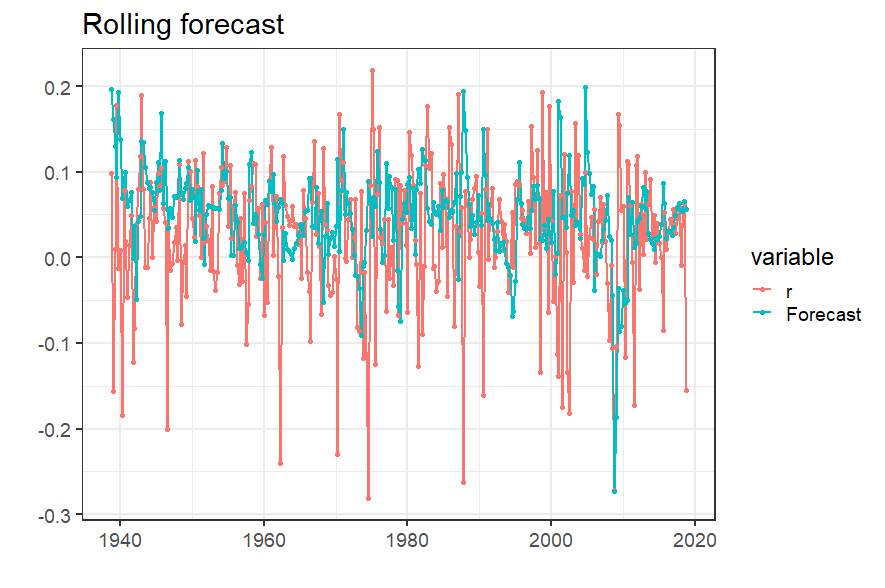
\includegraphics[scale = 0.5]{rolling_forecast.png}
	\caption{Rolling VAR forecast of returns}
	\label{fig:rolling_forecast}
\end{figure}

\end{document}

